\section{Алгоритми}

Тук ще докажем, че съществуват {\em полиномиални} алгоритми, които за дадена безконтекстна граматика $G$ проверяват:
\begin{itemize}
\item
  дали $\L(G) = \emptyset$;
\item
  дали $|\L(G)| = \infty$;
\item
  дали $|\L(G)| < \infty$;
\item
  по дадена дума $\alpha$ дали $\alpha \in \L(G)$.
\end{itemize}

\subsection{Опростяване на безконтекстни граматики}

\subsubsection*{Премахване на безполезните променливи}

Нека е дадена безконтекстната граматика $G = \CFG$.
\marginpar{\cite[стр. 88]{hopcroft1}}
Една променлива $A$ се нарича {\bf полезна}, ако съществува извод от следния вид:
\[S \to^\star_G \alpha A \beta \to^\star_G \gamma,\]
където $\gamma \in \Sigma^\star$, а $\alpha,\beta \in (V \cup \Sigma)^\star$.
Това означава, че една променлива е полезна, ако участва в извода на някоя дума в езика на граматиката.
Една променлива се нарича {\bf безполезна}, ако не е полезна.
Целта ни е да получим еквивалентна граматика $G'$ без безполезни променливи.
Ще решим задачата като разгледаме две леми.

\begin{lemma}
  \label{lem:useless1}
  Нека е дадена безконтекстната граматика $G$ и $\L(G) \neq \emptyset$.
  Съществува алгоритъм, който намира граматика $G'$, за която
  $\L(G) = \L(G')$ и със свойството, че  за всяка променлива $A' \in V'$, съществува дума $\alpha \in \Sigma^\star$,
  за която $A' \to^\star_{G'} \alpha$.
\end{lemma}
\begin{hint}
  Ще построим множествата
  \[V_n = \{A \in V \mid A \stackrel{\leq n}{\to}_G \alpha\ \&\ \alpha\in\Sigma^\star\}.\]

  \begin{itemize}
  \item
    Ясно е, че $V_0 = \emptyset$;
  \item
    Нека сме намерили $V_n$. Тогава
    \[V_{n+1} = V_n \cup \{A\in V \mid A \to_G \alpha\ \&\ \alpha \in (\Sigma \cup V_n)^\star \}.\]
  \item
    Когато намерим първото $n$, за което $V_n = V_{n+1}$,
    то знаем, че
    \[V_n = \{A \in V \mid A \to^\star_G \alpha\ \&\ \alpha \in \Sigma^\star \}.\]
    Дефинираме $G'$ като $V' = V_n$ и правилата на $G'$ са само тези правила на $G$, в които участват променливи от $V_n$ и букви от $\Sigma$.
  \end{itemize}
\end{hint}

\begin{cor}
  Съществува алгоритъм, който определя дали за всяка безконтекстна граматика $G$ дали $\L(G) = \emptyset$.
\end{cor}
\begin{proof}
  Прилагаме алгоритъма от \Lem{useless1}.
  Тогава $\L(G) = \emptyset$ точно тогава, когато $S \not\in V'$.  
\end{proof}

\begin{lemma}
  \label{lem:useless2}
  Съществува алгоритъм, който по дадена безконтекстна граматика $G = \CFG$, намира $G' = \pair{V',\Sigma',S,R'}$, $\L(G') = \L(G)$,
  със свойството, че за всяко $X \in V' \cup \Sigma'$ съществуват $\alpha, \beta \in (V'\cup\Sigma')^\star$,
  за които $S \to^\star \alpha X \beta$,
  т.е. всяка променлива или буква в $G'$ е достижима от началната променлива $S$.
\end{lemma}
\begin{hint}
  Строим множествата
  \begin{align*}
    & V_n = \{A \in V \mid S \stackrel{\leq n}{\to}_G \alpha A \beta\text{, за някои }\alpha,\beta \in (\Sigma \cup V)^\star\}\\
    & \Sigma_n = \{a \in \Sigma \mid S \stackrel{\leq n}{\to}_G \alpha a \beta\text{, за някои }\alpha,\beta \in (\Sigma\cup V)^\star\}.
  \end{align*}
  \begin{itemize}
  \item
    Ясно е, че $V_0 = \{S\}$ и $\Sigma_0 = \emptyset$.
  \item
    \marginpar{Всяка итерация отнема време $\mathcal{O}(|G|)$. Следователно, можем да намерим $G'$ за време $\mathcal{O}(|G|^2)$.}
    Нека имаме $V_n$ и $\Sigma_n$. Тогава:
    \begin{align*}
      & V_{n+1} = \{A \in V \mid (\exists B \in V_n)[ B \to_G \alpha A \beta\text{, за някои }\alpha,\beta \in (\Sigma\cup V)^\star]\}\\
      & \Sigma_{n+1} = \{a \in \Sigma \mid (\exists B \in V_n)[ B \to_G \alpha a \beta\text{, за някои }\alpha,\beta \in (\Sigma\cup V)^\star]\}.
    \end{align*}
  \item
    Спираме, когато намерим първото $n$, за което $V_n = V_{n+1}$ и $\Sigma_n = \Sigma_{n+1}$.
    Тогава $V' = V_n$ и $\Sigma' = \Sigma_n$.
  \end{itemize}
\end{hint}

\begin{thm}
  За всяка безконтекстна граматика $G$, за която $\L(G) \neq \emptyset$, съществува еквивалетнтна на нея безконтекстна граматика $G'$ без безполезни правила.
  Освен това, граматиката $G'$ може да се намери за полиномиално време.
\end{thm}
\begin{hint}
  \marginpar{Защо е важна последователността на прилагане?}
  Прилагаме върху $G$ първо процедурата от \Lem{useless1} и след това върху резултата прилагаме процедурата от \Lem{useless2}.
\end{hint}

\begin{example}
  Да разгледаме следната граматика $G$:
  \begin{align*}
    & S \to AB\ |\ aA\\
    & A \to a\ |\ aAa\\
    & B \to SB\ |\ BC\\
    & C \to \varepsilon\ |\ cC.
  \end{align*}
  Първо да намерим променливите, от които се извеждат думи.
  \begin{itemize}
  \item 
    $V_0 = \{A, C\}$, защото $A \to a$ и $C \to \varepsilon$;
  \item
    $V_1 = \{A, C, S\}$, защото $S \to aA$;
  \item
    не можем да добавим $B$ към $V_2$, следователно $V_1 = V_2$.
  \end{itemize}
  Получаваме граматиката $G'$:
  \begin{align*}
    & S \to aA\\
    & A \to a\ |\ aAa\\
    & C \to \varepsilon\ |\ cC.
  \end{align*}
  Сега премахваме променливите и буквите, които не са достижими от началната промелива $S$. Така получаваме граматиката $G''$:
  \begin{align*}
    & S \to aA\\
    & A \to a\ |\ aAa.
  \end{align*}
\end{example}

\begin{problem}
  Проверете дали $\L(G) = \emptyset$, където правилата на $G$ са:
  \begin{align*}
    & S \to AS\ |\ BC\\
    & A \to 0\ |\ BA\ |\ SB\\
    & B \to 1\ |\ BC\ |\ AB\\
    & C \to CB\ |\ SC\ |\ AS.
  \end{align*}
\end{problem}



%%% Local Variables:
%%% mode: latex
%%% TeX-master: "../eai"
%%% End:


\subsubsection*{Премахване на $\varepsilon$-правила}
\index{$\varepsilon$-правила}
За да премахнем правилата от вида $A \to \varepsilon$, следваме процедурата:
\marginpar{Броят на правилата може да се увеличи експоненциално, защото в най-лошия случай извеждаме всички подмножества на дадено множество от променливи}
\begin{enumerate}[1)]
\item 
  Намираме множеството $E = \{A \in V \mid A \to^\star \varepsilon\}$ по следния начин.
  Първо, $E := \{A \in V \mid A \to \varepsilon\}$.
  След това, за всяко правило от вида $B \to X_1\cdots X_k$, 
  ако всяко $X_i \in E$, то добавяме $B$ към $E$.
\item
  Строим множеството от правила $R'$, в което няма правила $\varepsilon$-правила по следния начин.
  За всяко правило $A \to x_1\cdots x_k$, където $x_i \in V\cup\Sigma$,
  добавяме към $R'$ всички правила от вида $A \to y_1\cdots y_k$, където:
  \begin{itemize}[-]
  \item 
    ако $x_i \not\in E$, то $y_i = x_i$;
  \item
    ако $x_i \in E$, то $y_i = x_i$ или $y_i = \varepsilon$;
  \item
    не всички $y_i$-та са $\varepsilon$.
  \end{itemize}
\end{enumerate}

\begin{example}
  Нека е дадена граматиката $G$ с правила
  \begin{align*}
    & S \to D\\
    & D \to AD\ |\ b\\
    & A \to AB\ |\ BC\ |\ a\\
    & B \to AA\ |\ UC\\
    & C \to \varepsilon\ |\ CA\ |\ a\\
    & U \to \varepsilon\ |\ aUb.
  \end{align*}
  % \[S\rightarrow D,D\rightarrow AD|b,A\rightarrow AB|BC|a, B\rightarrow AA|EC,C\rightarrow \varepsilon|CA|a, E\rightarrow \varepsilon|aEb.\]
  Тогава $E = \{X \in V \mid X \rightarrow^\star_G \varepsilon\} = \{A,B,C,U\}$.
  Това означава, че $\varepsilon \not\in \L(G)$.
  Граматиката $G'$ без $\varepsilon$-правила, за която $\L(G') = \L(G)$ има следните правила
  \begin{align*}
    & S \to D\\
    & D\to AD\ |\ D\ |\ b\\
    & A \to A\ |\ B\ |\ C\ |\ AB\ |\ BC\ |\ a\\
    & B\to A\ |\ E\ |\ C\ |\ AA\ |\ UC\\
    & C \to C\ |\ A\ |\ CA\ |\ a\\
    & U \to aUb\ |\ ab.
  \end{align*}
\end{example}

%%% Local Variables:
%%% mode: latex
%%% TeX-master: "../eai"
%%% End:


\subsubsection*{Премахване на преименуващи правила}
\index{преименуващи правила}
Преименуващите правила са от вида $A \to B$.
Нека е дадена граматика $G = \CFG$.
Ще построим еквивалентна граматика $G'$ без преименуващи правила.
В началото нека в $R'$ да добавим всички правила от $R$, които не са преименуващи.
След това, за всякa променлива $A$, за която $A \derive{\star}_G B$,
ако $B \to \alpha$ е правило в $R$, което не е преименуващо,
то добавяме към $R'$ правилото $A \to \alpha$.

\begin{lemma}
  Съществува {\em полиномиален} алгоритъм, такъв че превръща всяка безконтекстна граматика $G$ в безконтекстна граматика $G'$ без преименуващи правила
  и $\L(G') = \L(G) \setminus \{\varepsilon\}$.
\end{lemma}
\begin{hint}
  Първо намираме множеството от двойки
  \[\texttt{Ren} = \{(A,B) \in V\times V \mid A \derive{\star} B\}\]
  като строим множествата по такъв начин, че:
  \[\texttt{Ren[n]} = \{(A,B) \in V\times V \mid A \derive{\leq n} B\}\]

  \begin{align*}
    & \texttt{Ren[0]} \df \{(A,A) \mid A \in V\}\\
    & \texttt{Ren[n+1]} \df \texttt{Ren[n]} \cup \{(A,B) \mid (\exists C)[ A \to_G C\ \&\ (C,B) \in \texttt{Ren[n]}]\}.
  \end{align*}
  
  % \begin{itemize}
  % \item
  %   % Ясно е, че $\texttt{Ren[0]} \df \{(A,A) \mid A \in V\}$.
  %   $
  % \item
  %   Нека имаме $\texttt{Ren[n]}$. Тогава дефинираме
  %   \mynote{Всяка итерация отнема $\mathcal{O}(|G|)$ време.}
  %   \[\texttt{Ren[n+1]} \df \texttt{Ren[n]} \cup \{(A,B) \mid (\exists C)[ A \to_G C\ \&\ (C,B) \in \texttt{Ren[n]}]\}.\]
  % \item
  \mynote{$|\texttt{Ren}|$ има големина $\mathcal{O}(|G|^2)$.}
  Спираме на първото $n$, за което $\texttt{Ren[n]} = \texttt{Ren[n+1]}$. Тогава $\texttt{Ren} = \texttt{Ren[n]}$.
  % \end{itemize}
  
  Нека $R'_0 \df R \setminus (V\times V)$ са правилата на $R$, които не са преименуващи. Тогава
  \[R' \df  \{\ (A,\alpha) \in V \times (V\cup\Sigma)^\star \mid (\exists B)[(A,B) \in \texttt{Ren}\ \&\ (B,\alpha) \in R'_0]\ \}.\]
\end{hint}

% \ExtraMaterial{
\begin{extra}
\begin{multicols}{2}
    \begin{example}
      Нека е дадена граматиката $G$ с правила  
      \begin{align*}
        & S \to B\ |\ CC\ |\ b\\
        & A \to S\ |\ SB\\
        & B \to C\ |\ BC\\
        & C \to AB\ |\ a\ |\ b.
      \end{align*}
      Да намерим първо $\texttt{Ren}$.
      \begin{align*}
        \texttt{Ren[0]} = \{ & (S,S), (A,A), (B,B), (C,C)\};\\
        \texttt{Ren[1]} = \{ & (S,S), (S,B), (A,A), (A,S),\\
                             & (B,B), (B,C), (C,C)\};\\
        \texttt{Ren[2]} = \{ & (S,S),(S,B), (S,C), (B,B), (B,C),\\
                             & (C,C), (A,A), (A,S), (A,B)\};\\
        \texttt{Ren[3]} = \{ & (S,S),(S,B), (S,C), (B,B), (B,C),\\
                             & (C,C), (A,A), (A,S), (A,B), (A,C)\};\\
        \texttt{Ren[4]} = \{ & (S,S),(S,B), (S,C), (B,B), (B,C),\\
                             & (C,C), (A,A), (A,S), (A,B), (A,C)\};\\
      \end{align*}
      
      Получихме, че $\texttt{Ren[3]} = \texttt{Ren[4]}$.
      Оттук можем да заключим следното:
      \begin{align*}
        & A \derive{\star} A,B,S,C\\
        & B \derive{\star} B,C\\
        & S \derive{\star} S,B,C\\
        & C \derive{\star} C.          
      \end{align*}
      % \end{itemize}
      
      Първо добавяме към $R'$ правилата, които не са преименуващи, а именно:
      \begin{align*}
        & A \to BS\\
        & B \to BC\\
        & C \to AB\ |\ a\ |\ b\\
        & S \to CC\ |\ b.
      \end{align*}
      \begin{itemize}
      \item 
        Понеже имаме,че $A \derive{\star} B,S,C$, то добавяме към $R'$ правилата:
        \[A \to BC\ |\ AB\ |\ a\ |\ b\ |\ CC.\]
      \item
        Понеже имаме,че $B \derive{\star}_G C$, то добавяме към $R'$ правилата:
        \[B \to AB\ |\ a\ |\ b.\]
      \item
        Понеже имаме, че $S \derive{\star}_G B,C$, то добавяме към $R'$ правилата:
        \[S \to BC\ |\ AB\ |\ a\ |\ b.\]
      \end{itemize}
      Накрая получаваме, че граматиката $G'$ има правила
      \begin{align*}
        & S \to BC\ |\ AB\ |\ CC\ |\ a\ |\ b\\
        & A \to BS\ |\ BC\ |\ AB\ |\ a\ |\ b\ |\ CC\\
        & B \to AB\ |\ a\ |\ b\ |\ BC\\
        & C \to AB\ |\ a\ |\ b.
      \end{align*}
    \end{example}
  \end{multicols}
\end{extra}

\begin{extra}
\begin{problem}
  Премахнете преименуващите правила от граматиката $G$, като запазите езика, ако $G$ има следните правила:
    \begin{align*}
      & S \to C\ |\ CC\ |\ b\\
      & A \to B\\
      & B \to S\ |\ C\ |\ BC\\
      & C \to a\ |\ AB;
    \end{align*}
\end{problem}
\end{extra}

%%% Local Variables:
%%% mode: latex
%%% TeX-master: "../eai"
%%% End:


\subsubsection*{Премахване на дългите правила}

Едно правило се нарича дълго, ако е от вида $A \to \beta$, където $|\beta| \geq 3$.
Да разгледаме едно дълго правило в граматиката от вида $A \to x_1x_2\cdots x_k$, 
където $k \geq 3$ и $x_i \in V \cup \Sigma$. За да получим еквивалентна граматика без това дълго правило,
добавяме нови променливи $A_1,\dots, A_{k-2}$, и правила
\[A \to x_1A_1,\ A_1 \to x_2A_2, \dots,\ A_{k-2} \to x_{k-1}x_k.\]


\begin{problem}
  Нека е дадена граматиката  $G = \pair{\{S,A,B,C\}, \{a,b\}, S, R}$.
  Използвайте обща конструкция, за да премахнете ,,дългите'' правила от $ G$ като при това получите 
  безконтестна граматика $G_1$ с език $\L(G) = \L(G_1)$, където правилата на граматиката са:
  % \begin{enumerate}[a)]
  % \item
  %   \begin{align*}
  %     & S \to \varepsilon\ |\ ab\ |\ aAba\\
  %     & A\to aBCb\\
  %     & B\to bbb\\
  %     & C\to aC\ |\ aCaC;
  %   \end{align*}
  % \item
    \begin{align*}
      & S\to CC\ |\ b\\
      & A\to BSB\ |\ a\\
      & B\to ba\ |\ BC\\
      & C\to BaSA\ |\ a\ |\ b.
    \end{align*}
  % \end{enumerate}
\end{problem}

%%% Local Variables:
%%% mode: latex
%%% TeX-master: "../eai"
%%% End:


\subsection{Нормална Форма на Чомски}
\index{Чомски}
%[стр. 99 от \cite{sipser}]
\index{нормална форма на Чомски}
Една безконтекстна граматика е в {\bf нормална форма на Чомски}, ако
всяко правило е от вида
\[A \rightarrow BC\mbox{ и }A \rightarrow a,\]
където $A, B, C$ са произволни променливи и $a$ е произволна буква.
\mynote{Ако искаме $\varepsilon$ да бъде в езика на граматиката, то позволяваме от началната променлива $S$ да имаме правилото $S \to_G \varepsilon$,
но тогава забраняваме $S$ да се среща в дясна страна на правило.}
% Освен това, позволяваме правилото $S\to\varepsilon$.
% \footnote{В \cite[стр. 151]{papadimitriou} дефиницията е малко по-различна.
% Там дефинират $G$ да бъде в нормална форма на Чомски ако $R \subseteq V\times(V\cup\Sigma)^2$.
% В този случай губим езиците $\{\varepsilon\}$ и $\{a\}$, за $a\in\Sigma$.}

\begin{framed}
  \begin{theorem}
    Всеки безконтекстен език $L$, който не съдържа $\varepsilon$, се поражда от безконтекстна граматика в нормална форма на Чомски.
  \end{theorem}
\end{framed}
\begin{proof}
%  \marginpar{Броят на правилата може да се увеличи експоненциално.}
  Нека имаме безконтекстна граматика $G$, за която $L = \L(G)$.
  Ще построим безконтекстна граматика $G^\prime$ в нормална форма на Чомски, $L = \L(G^\prime)$.
  % [стр. 99 от \cite{sipser}]
  Следваме следната процедура:
  \begin{itemize}
  \item
    Премахваме дългите правила.
    Това можем да направим за време $\mathcal{O}(|G|)$
    като новата граматика ще има дължина $\mathcal{O}(|G|)$.
  \item
    \mynote{Редът на стъпките е важен. Трябва преди това сме премахнали дългите правила. Вижте \cite[стр. 296]{hopcroft2}.}
    Премахваме $\varepsilon$-правилата.
    Това можем да направим за време $\mathcal{O}(|G|^2)$
    като новата граматика ще има дължина $\mathcal{O}(|G|)$.
  \item
    Премахваме преименуващите правила.
    Това можем да направим за време $\mathcal{O}(|G|^2)$
    като новата граматика ще има дължина $\mathcal{O}(|G|^2)$.
  \item
    За правила от вида $A\to u_1 u_2$, където $u_1, u_2 \in V \cup \Sigma$, 
    заменяме всяка буква $u_i$ с новата променлива $U_i$
    и добавяме правилото $U_i\to u_i$.
    Например, правилото $A \to aB$ се заменя с правилото $A \to XB$ и добавяме правилото $X \to a$,
    където $X$ е нова променлива.
    Това можем да направим за време $\mathcal{O}(|G|)$ и новата граматика ще има дължина $\mathcal{O}(|G|)$.
  \item
    Ако искаме $\varepsilon$ да бъде в езика на граматиката, то добавяме нова начална променлива $S_0$
    и правило $S_0 \to_G \varepsilon$ и правилата $S_0 \to \alpha$ за $S \to \alpha$.
  \end{itemize}
\end{proof}

\begin{theorem}
  При дадена безконтекстна граматика $G$, можем да намерим еквивалентна
  на нея граматика $G'$ в нормална форма на Чомски за време $\mathcal{O}(|G|^2)$,
  като получената граматика е с дължина $\mathcal{O}(|G|^2)$.
\end{theorem}

\begin{theorem}
  \mynote{\cite[стр. 137]{hopcroft1}. Важно е, че алгоритмът е полиномиален.
    \writedown Защо от \Lemma{pumping-context} имаме експоненциален алгоритъм за проверка дали езикът на една граматика е безкраен?}
  Съществува \emph{полиномиален} алгоритъм, който определя по дадена безконтекстна граматика $G$ дали $\L(G)$ е безкраен език.
\end{theorem}
\begin{proof}
  Нека е дадена една безконтекстна граматика $G$.
  Нека да разгледаме граматиката $G'$ в НФЧ {\em без безполезни променливи}, за която $\L(G) = \L(G')$.
  От граматиката $G' = \pair{V',\Sigma,S,R'}$ строим граф с възли променливите от $V'$ като
  за $A,B \in V'$ имаме ребро $A \to B$ в графа точно тогава, когато съществува $C \in V'$,
  за което $A \to_{G'} BC$ или $A \to_{G'} CB$ е правило в граматиката $G$.
  Сега ще съобразим, че ако в получения граф имаме цикъл, то $\L(G') = \infty$.
  Да разгледаме един такъв цикъл в графа:
  \[A_0 \to A_1 \to A_2 \to \cdots \to A_n \to A_0.\]
  Понеже граматиката е в нормална форма на Чомски, то същестуват думи $\lambda,\rho \in (V\cup\Sigma)^\star$, за които $A_0 \yield{n+1} \lambda A_0 \rho$ и $\abs{\lambda\rho} = n+1$

  \begin{figure}[H]
    \begin{subfigure}[t]{0.5\textwidth}
    \centering
      \begin{tikzpicture}[scale=0.8]
      \node (A) at (0,0) {\footnotesize{$A_0$}};
      \coordinate (B) at (-2,-3);
      \coordinate (C) at (2,-3);
      \node (D) at (0,-1.2) {\footnotesize{$A_i$}};
      \coordinate (D1) at (1.4,-3);
      \coordinate (D2) at (-1.4,-3);
      \node (E) at (0,-2.3) {\footnotesize{$A_n$}};
      \coordinate (E1) at (0.7,-3);
      \coordinate (E2) at (-0.7,-3);
      \coordinate (F) at (0,-3);

      \draw (A) -- node[above left]{$P = $} (B) -- node[below]{$A_0$}(C) -- (A);
      \draw [photon] (A) -- (D) -- (E) -- (F);
    \end{tikzpicture}
    \caption{$A_0 \yield{n+1} \lambda A_0 \rho$, където $\lambda, \rho \in (V\cup\Sigma)^\star$.}
    \end{subfigure}
    ~ 
    \begin{subfigure}[t]{0.5\textwidth}
      \centering
      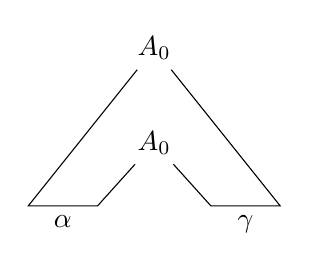
\begin{tikzpicture}[scale=0.8]
        \node (A) at (0,0) {$A_0$};
        \coordinate (B) at (-2,-2.5);
        \coordinate (C) at (2,-2.5);
        \coordinate (D) at (-0.9,-2.5);
        \coordinate (E) at (0.9,-2.5);
        \node (F) at (0,-1.5) {$A_0$};
        \draw (A) -- (B) -- node[below]{$\alpha$} (D) -- (F) -- (E) -- node[below]{$\gamma$} (C) -- (A);
      \end{tikzpicture}
      \caption{$A_0 \yield{\geq n+1}\alpha A_0\gamma$, където $\alpha,\gamma \in \Sigma^\star$.}
    \end{subfigure}
  \end{figure}

  Понеже в $G$ няма безполезни променливи, то $\lambda \derive{\star} \alpha$, където $\alpha \in \Sigma^\star$ и $\abs{\lambda} \leq \abs{\alpha}$ и $\rho \derive{\star} \gamma$,
  където $\gamma \in \Sigma^\star$ и $\abs{\rho} \leq \abs{\gamma}$.
  Оттук заключаваме, че $A_0 \yield{\star} \alpha A_0 \gamma$ и $\abs{\alpha\gamma} \geq 1$.
  Понеже $A_0$ не е безполезна променлива, то $A_0 \yield{\star} \beta$, за някоя дума $\beta \in \Sigma^\star$.
  Сега комбинираме \Proposition{pumping:ground} и \Proposition{pumping:iteration} за да получим следния извод:
  \begin{prooftree}
    \AxiomC{$A_0 \yield{\star} \alpha A_0 \gamma$}
    \AxiomC{$A_0 \yield{\star} \beta$}
    \AxiomC{$i \in \Nat$}
    \TrinaryInfC{$A_0 \yield{\star} \alpha^i \beta \gamma^i$}
  \end{prooftree}
  Понеже $\abs{\alpha\beta} \geq 1$, заключаваме, че $\L(G)$ е безкраен език.
  Така доказахме, че ако в графът има цикли, то $\L(G)$ е безкраен език.
  
  За обратната посока, нека в графът няма цикли.
  Да разгледаме една променлива $A$, от която най-дългият път има $k$ на брой възли.
  От принципа на Дирихле знаем, че $k \leq \abs{V}$.
  Това означава, че ако $A \yield{\star} \alpha$, за някоя $\alpha \in \Sigma^\star$,
  то $A \yield{\leq k} \alpha$ и понеже граматиката е в нормална форма на Чомски,
  то $\abs{\alpha} \leq 2^{k-1}$.
  Оттук следва, че всички думи, които се извеждат от променливата $A$ са най-много $2^{k-1}$ на брой.
  Заключаваме, че ако в графът няма цикли, то $\L(G)$ е краен.
\end{proof}

\begin{theorem}
  Съществува \emph{полиномиален} алгоритъм, който определя по дадена безконтекстна граматика $G$ дали $\L(G)$ е краен език.
\end{theorem}

%%% Local Variables:
%%% mode: latex
%%% TeX-master: "../eai"
%%% End:


\subsection{Проблемът за принадлежност}

\begin{thm}
  Съществува {\em полиномиален} алгоритъм относно дължината на входната дума, който проверява дали дадена дума принадлежни на граматиката $G$.
  \marginpar{За дума $\alpha$, алгоритъмът работи за време $O(\abs{\alpha}^3)$}
\end{thm}
% \begin{proof}[стр. 154 от \cite{papadimitriou}]
Можем да приемем, че $G = \CFG$ е граматика в нормална форма на Чомски.
Нека $\alpha = a_1a_2\dots a_n$ е дума, за която искаме да проверим дали $\alpha \in \L(G)$.
\marginpar{Това е алгоритъм на Cocke, Younger и Kasami (CYK), които откриват идеята за този алгоритъм независимо. Той е пример за динамично програмиране \cite[стр. 192]{kozen}}
\begin{algorithm}[H]
  \caption{Проверка дали $\alpha \in \L(G)$}
  \label{alg:belongs-to-grammar}
  \begin{algorithmic}[1]
    \State $n := \abs{\alpha}$ \Comment{Вход дума $\alpha = a_1\cdots a_n$}
    \ForAll{$i\in [1,n]$}
    \State $V[i,i] := \{A \in V \mid A\to_G a_i\}$
    \EndFor
    \ForAll{$i,j \in [1,n]\ \&\ i \neq j$}
    \State $V[i,j] := \emptyset$
    \EndFor      
    \ForAll{$s \in [1, n)$} \Comment{Дължина на интервала}
    \ForAll{$i \in [1, n-s]$}\Comment{Начало на интервала}
    \ForAll{$k \in [i, i + s)$}\Comment{Разделяне на интервала}
    \If{$\exists A\to BC \in R\ \&\ B \in V[i,k]\ \&\ C\in V[k+1,i+s]$}
    \State $V[i,i+s] := V[i,i+s] \cup \{A\}$
    \EndIf
    \EndFor
    \EndFor
    \EndFor
    \If{$S \in V[1,n]$}
    \State \Return \texttt{True}\Comment{Има извод на думата от $S$}
    \Else
    \State \Return \texttt{False}
    \EndIf
  \end{algorithmic}
\end{algorithm}

\begin{lemma}
  За дадена граматика в нормална форма на Чомски и дума $\alpha$, 
  за всяко $0 \leq s < \abs{\alpha}$, след $s$-тата итерация на алгоритъма (редове 6 - 10), за всяка позиция $i = 1,\dots,n-s$,
  \[V[i,i+s] = \{A \in V \mid A \rightarrow^\star_G a_i\dots a_{i+s}\}.\]
\end{lemma}
\begin{proof}
  Пълна индукция по $s$.
  За $s = 0$ е ясно, защото от редове 2 и 3 и от факта, че граматиката е в НФЧ следва, че за всяко $i = 1, \dots, n$,
  \[V[i,i] = \{A \in V \mid A \to_G a_i\} = \{A \in V \mid A \to^\star_G a_i\}.\]

  Нека твърдението е вярно за $s < n$. Ще докажем твърдението за $s+1$, т.е. ще докажем, че за всяко $i = 1,\dots,n-s-1$
  е изпълнено, че:
  \[V[i,i+s+1] = \{A \in V \mid A \rightarrow^\star_G a_i\dots a_{i+s+1}\}.\]
  Да разгледаме двете посоки на това равенство.
  % Да разгледаме $A \in V[i,i+s+1]$.
  \begin{description}
  \item[($\subseteq$)]
    Нека $A \in V[i,i+s+1]$.
    Единствената стъпка на алгоритъма, при която може да сме добавили $A$ към множеството $V[i,i+s+1]$ е ред 10.
    Тогава имаме, че съществува $k \geq i$, за което $B \in V[i,k]$, $C \in V[k+1,i+s+1]$, и $A\to_G BC$.
    Понеже $k-i < s+1$ и $i+s+1 - k - 1 < s+1$, от {\bf И.П.} имаме, че $B \to^\star_G a_i\cdots a_k$ и $C \to^\star_G a_{k+1}\cdots a_{i+s+1}$.
    Заключаваме веднага, че 
    \[A \to^\star_G a_i\cdots a_{i+s+1}.\]
  \item[($\supseteq$)]
    Нека $A \to^\star_G a_i\cdots a_{i+s+1}$ и да разгледаме първото правило, което сме приложили в този извод.
    Понеже $G$ е в нормална форма на Чомски, правилото е от вида $A \to_G BC$ и тогава съществува някое $t < s+1$, за което 
    $B \to^\star a_i\cdots a_{i+t}$ и $C \to^\star a_{i+t+1}\cdots a_{i+s+1}$.
    От {\bf И.П.} получаваме, че $B \in V[i,i+t]$ и $C \in V[i+t+1,i+s+1]$.
    Тогава от ред 10 на алгоритъма е ясно, че 
    \[A \in V[i,i+s+1].\]
  \end{description}
\end{proof}

\begin{example}
  Нека е дадена граматиката $G$ с правила 
  \begin{align*}
    & S\rightarrow a\ |\ AB\ |\ AC\\
    & A\rightarrow a\\
    & B\rightarrow b\\
    & C\rightarrow SB\ |\ AS.
  \end{align*}
  Ще приложим $CYK$ алгоритъма за да проверим дали думата $aaabb \in \L(G)$.
  \begin{itemize}
  \item 
    За $s = 0$ имаме, че:
    \begin{itemize}
    \item 
      $V[1,1] = V[2,2] = V[3,3] = \{S,A\}$;
    \item
      $V[4,4] = V[5,5] = \{B\}$.
    \end{itemize}
  \item
    За $s = 1$ имаме, че:
    \begin{itemize}
    \item
      $V[1,2] = V[2,3] = \{C\}$;
    \item
      $V[3,4] = \{S,C\}$;
    \item
      $V[4,5] = \emptyset$.
    \end{itemize}
  \item
    За $s = 2$ имаме, че:
    \begin{itemize}
    \item
      $V[1,3] = \{S\} \cup \emptyset$;
    \item
      $V[2,4] = \{S,C\} \cup \emptyset$;
    \item
      $V[3,5] = \emptyset \cup \{C\}$.
    \end{itemize}
  \item
    За $s = 3$ имаме, че:
    \begin{itemize}
    \item
      $V[1,4] = \{S,C\} \cup \emptyset \cup \emptyset = \{S,C\}$;
    \item
      $V[2,5] = \{S\} \cup \emptyset \cup \{C\} = \{S,C\}$.
    \end{itemize}
  \item
    За $s = 4$ имаме, че:
    \begin{itemize}
    \item 
      $V[1,5] = \{S,C\} \cup \emptyset \cup \emptyset \cup \{C\}= \{S,C\}$.
    \end{itemize}
  \end{itemize}
  Понеже $S \in V[1,5]$, то $aaabb \in \L(G)$.
\end{example}


%%% Local Variables:
%%% mode: latex
%%% TeX-master: "../eai"
%%% End:


%%% Local Variables: 
%%% mode: latex
%%% TeX-master: "../eai"
%%% End: 
